\subsection*{Part C}

\textit{Discuss why the Transformer architecture has been crucial for applying language modelling to very large datasets and in effectively capturing long range dependencies. Support your discussion by citing specific sections or experiments from at least TWO (2) recent peer-reviewed papers.}

\begin{center}
  $\ast$~$\ast$~$\ast$
\end{center}

Resources sourced from lectures videos published by one of the Professor in National Taiwan University, Hung-yi Lee with title: \textbf{[Generative AI] Large Models + Large Dataset = Magnificent Results?}

\begin{itemize}
    \item \url{https://www.youtube.com/watch?v=SaZTJJNOCOY}
    \item \url{https://www.youtube.com/watch?v=qycxA-xX_OY}
    \item \url{https://www.youtube.com/watch?v=V-3ksGCjehU}
\end{itemize}

Transformer architecture has emerged as a cornerstone in the evolution of language modeling, particularly when dealing with extensive datasets. Its prominence is attributed to inherent efficiencies in parallel processing and a robust capacity for capturing long-range dependencies within textual data. These characteristics have facilitated significant advancements in the scale and performance of language models.

\begin{figure}[htpb]
    \centering
    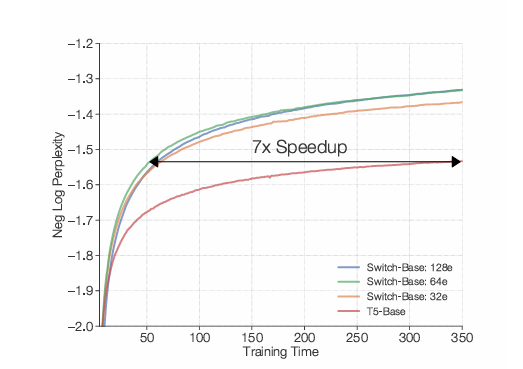
\includegraphics[width=0.6\textwidth]{../images/image-3.png} % Replace with your image path
    \caption{Speed advantage of Switch Transformer. All models trained on 32 TPUv3 cores with equal FLOPs per example. For a xed amount of computation and training time, Switch Transformers signi cantly outperform the dense Transformer baseline. Our 64 expert Switch-Base model achieves the same quality in one-seventh the time of the T5-Base and continues to improve}
    \label{fig:switch}
\end{figure}

A critical advantage of the Transformer architecture lies in its remarkable scalability and proficiency in managing large datasets. The architecture's self-attention mechanism is central to this capability, permitting the simultaneous processing of all tokens in an input sequence. This parallelism contrasts sharply with recurrent neural networks (RNNs), which process token sequentially, and is indispensable for the efficient training of contemporary language models on massive data corpora. Research by \parencite{kaplan_scaling_2020} established that model performance demonstrates a power-law relationship with model size, dataset size, and computational resources, and the Transformer architecture is pivotal in realizing such scaling. Building on this, \parencite{fedus_switch_2022} introduced sparsity through Switch Transformers, enabling the efficient training of models with over a trillion parameters. Their work highlighted that the Switch Transformer architecture could achieve up to a sevenfold increase in pre-training speed using equivalent computational resources by effectively leveraging hardware designed for dense matrix multiplications, thereby maximizing parameter count in a computationally efficient manner as shown in Fig \ref{fig:switch}. Further underscoring the importance of data and model scaling, \parencite{hoffmann_training_2022} determined that optimal training necessitates a proportional scaling of both model size and the number of training tokens, reinforcing the need for architectures like Transformers that can effectively process vast quantities of data. The practical manifestation of this scalability is exemplified by models such as Gopher, a 280 billion parameter model discussed by \parencite{rae_scaling_2022}, which showcases the Transformer's capacity to handle extremely large model dimensions as shown in Fig \ref{fig:gopher}.

\begin{figure}[htpb]
    \centering
    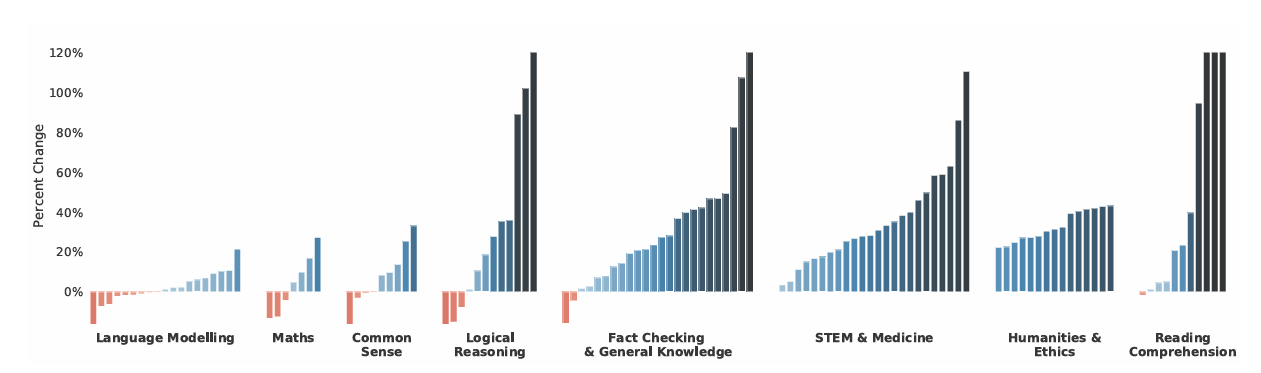
\includegraphics[width=0.6\textwidth]{../images/image-4.png} % Replace with your image path
    \caption{An overview of the percentage change in performance metric (higher is better) of Gopher versus state-of-the-art language model performance across 124 tasks. Each bar represents a task, here we clip the maximum relative improvement to 120\%. In total Gopher shows an improvement across 100 / 124. The best-published results include (175B) GPT-3, (178B) Jurassic-1, and (530B) Megatron-Turing NLG.}
    \label{fig:gopher}
\end{figure}

Beyond scalability, the Transformer's proficiency in capturing long-range dependencies—relationships between distant tokens in a sequence—is fundamental to its success. This ability is crucial for comprehending context and generating coherent, meaningful text. The self-attention mechanism allows each token to directly attend to all other tokens in the sequence, irrespective of their proximity. This direct pathway for information flow overcomes a significant limitation of RNNs, where information must traverse numerous intermediate steps, risking issues like vanishing gradients. While the foundational concept was introduced by \parencite{vaswani_attention_2023}, the empirical success of large-scale models such as Gopher and those analyzed by \parencite{kaplan_scaling_2020} across diverse tasks implicitly validates the Transformer's strength in this domain. These models consistently achieve high performance on tasks demanding deep contextual understanding, which inherently relies on the effective capture of long-range dependencies.

\begin{figure}[htpb]
    \centering
    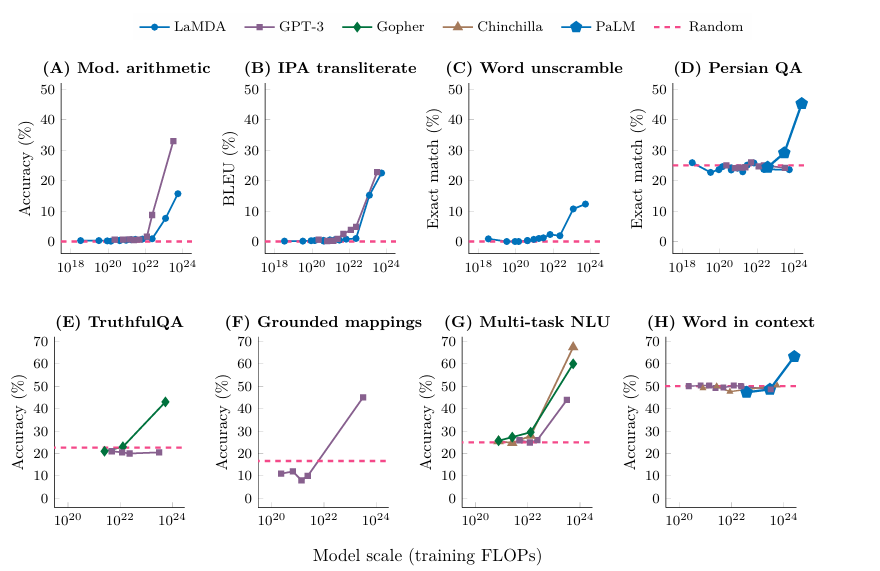
\includegraphics[width=0.8\textwidth]{../images/image.png} % Replace with your image path
    \caption{Model Scaling: Eight examples of emergence in the few-shot prompting setting. Each point is a separate model.The ability to perform a task via few-shot prompting is emergent when a language model achieves random performance until a certain scale,after which performance significantly increases to well-above random.Note that models that used more training compute also typically have more parameters—hence,we show ananalogous figure with number of model parameters instead of training FLOPs as the x-axis}
    \label{fig:model_scaling}
\end{figure}

\begin{figure}[htpb]
    \centering
    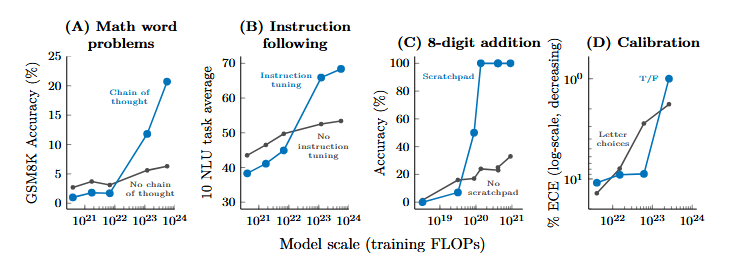
\includegraphics[width=0.5\textwidth]{../images/image-1.png} % Replace with your image path
    \caption{Augmented Prompting: Specialized prompting or finetuning methods can be emergent in that they do not have a positive
 effect until a certain model scale.}
    \label{fig:augmendted_prompting}
\end{figure}

\begin{figure}[htpb]
    \centering
    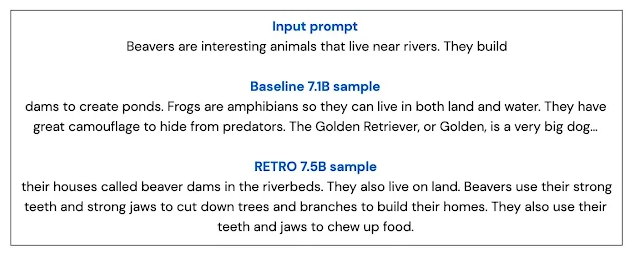
\includegraphics[width=0.6\textwidth]{../images/image-2.png} % Replace with your image path
    \caption{The RETRO model stays more on-topic than the baseline sample.Type image caption here (optional)}
    \label{fig:retro}
\end{figure}

The significance of this capability is further evidenced by the emergence of complex reasoning abilities in large-scale models. \parencite{wei_emergent_2022} discuss how phenomena like multi-step reasoning, often facilitated by techniques such as chain-of-thought prompting, become apparent in models typically exceeding 100 billion parameters as seen in Fig \ref{fig:model_scaling} and Fig \ref{fig:augmendted_prompting}. Such reasoning abilities frequently depend on understanding relationships across extended textual contexts, a feat well-supported by the Transformer architecture. Innovations like RETRO (Retrieval-Enhanced Transformer), introduced by \parencite{borgeaud_improving_2021}, augment Transformers with external retrieval mechanisms to enhance factuality and topical coherence. While retrieval provides supplementary information, the core Transformer architecture remains responsible for processing both the input and the retrieved passages, adeptly integrating their long-range contextual relationships as seen from Fig \ref{fig:retro}. Similarly, \parencite{khandelwal_generalization_2020} demonstrated that augmenting a pre-trained Transformer language model with a k-nearest neighbors model can improve predictions, particularly for rare patterns and factual knowledge, which often hinge on specific long-range contextual cues.

In summary, the continuous development and refinement of Transformer-based models, encompassing innovations like Switch Transformers for enhanced sparsity and retrieval-augmented models such as RETRO, underscore the fundamental strengths of this architecture. Its dual capabilities—efficient training on vast datasets and the inherent capacity to model complex, long-range relationships within text—have solidified the Transformer as the predominant backbone of modern large-scale language modeling. Ongoing research into areas such as instruction tuning \parencite{tay_long_2021,chung_scaling_2022}, model calibration, and more nuanced understanding of scaling behaviors, as seen in the work by \parencite{wei_emergent_2022} on emergent abilities, continues to build upon this powerful foundation, often seeking to more effectively train or adapt existing Transformer-based systems.
